\begin{figure}[htb]
\centering
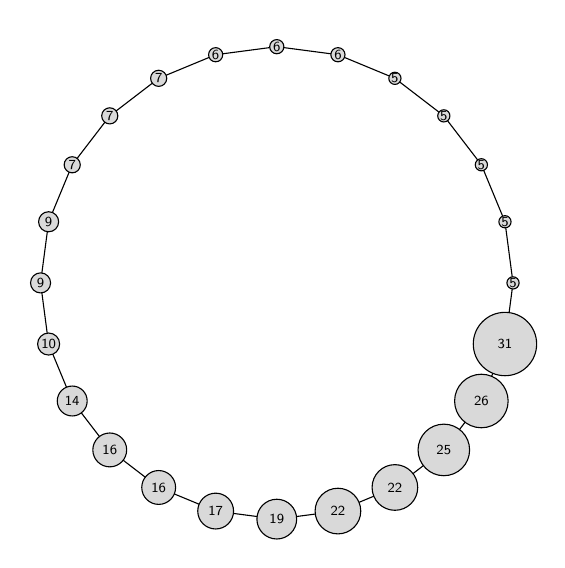
\begin{tikzpicture}
\def\cradius{3.0};
%\draw[help lines,step=1] (0,-5) grid (10,5);
\edef\counter{0};
%\def\sizes{{ 4, 4, 4, 9, 15, 17, 45, 52}};
\def\sizes{{5, 5, 5, 5, 5, 6, 6, 6, 7, 7, 7, 9, 9, 10, 14, 16, 16, 17, 19, 22, 22, 25, 26, 31}};

\draw (0:\cradius)
\foreach \x in {0,15,...,345}{ -- (\x:\cradius) }-- cycle (90:\cradius) node[above] {};

\foreach \angle in {0,15,...,345}{
      \def\cliquer{ {\angle * 0.002} };
      
      \pgfmathsetmacro{\pg}{\sizes[\counter]}; % set the macro pg with the current value of counter
      \counter
      \fill[draw, fill=gray!30] (\angle:\cradius) circle (\pg * 0.0125+0.015);
      %\draw[fill=gray!30] (\angle:\cradius) circle [radius=0.1];
      \node[black] at (\angle:3) {{\tiny $\mathsf{{\pg}}$}};
      \pgfmathparse{\counter + 1}; \xdef\counter{\pgfmathresult}; % increment counter and store the result again in counter
      }
\end{tikzpicture}
\caption{Power-law ring of cliques. Every circle is a complete graph (clique). Every clique is connected to its neighbors with one single link. The sizes of the cliques are randomly sampled from a power-law distribution with minimum clique size $\min_c=5$, maximum clique size $\max_c=75$, $n=150$, $\tau_c=1$.}
\label{fig:ring_of_clique_powerlaw}
\end{figure}